\section{Tests}
\subsection{Unit Tests}

\subsection{Hydro Tests}
\subsubsection{Linear Wave}
Sound waves provide the mechanism to transport disturbances in a fluid. An
elementary test problem is the ability maintain wave propagation of small
disturbances. Given a fluid in equilibrium with constant density $\rho_0$,
pressure $P_0$ and zero velocity $\mathbf{v}=0$ with perturbations of the form
\begin{equation}
	\begin{array}{rcl}
		\rho & = & \rho_0 + \delta\rho(x,t) \\
   		 P & = & P_0 + \delta p(x,t) \\
    	\mathbf{v} & = & \delta\mathbf{v}(x,t),
    \end{array}
\end{equation}
and maintaining terms to first order in the Euler equations produce the wave
equation for each variable with a wave propagation speed equal to the fluid's sound speed 
$c_s$. Thus, setting a small disturbance 
will propagate with a finite velocity maintaining its form as along as the initial
disturbances are relatively small.

We set up a 2d box of unit length with constant $\rho_0=1.0$, $P_0=3/5$, $\mathbf{v}=0$,
and $\gamma=5/3$ with periodic boundary conditions. A sinusoidal wave in the x direction of 
the form $\delta\rho(x,t) = Asin(kx + wt)$ with $k=w=2\pi$ and $A=10^{-6}$ is added at time 
$t=0$. The remaining disturbances can be specified through $\delta\rho$ by the following
\begin{equation}
	\begin{array}{rcl}
        \delta \mathbf{v}(x,0) & = & \left(\frac{w}{k}\right)\delta
        	\rho(x,0)/\rho_0\mathbf{\hat{x}}\\
        \delta P(x,0) & = & \left(\frac{w}{k}\right)^2\delta\rho(x,0).
    \end{array}
\end{equation}
The values chosen produce waves traveling rightward with a velocity of 1. The simulation is
evolved for 1 time unit such that the waves return to its' initial position at time $t=0$. 
Moreover, we study the convergence behavior by comparing the final state of the density to 
the initial density by computing the $L1$ norm,
\begin{equation}
	L1 = \frac{1}{N^2}\sum_i \left| \rho_i - \rho(x_i) \right|,
\end{equation}
where $\rho_i$ is final density at position $x_i$ and $\rho(x_i)$ is the density at t=0
at position $x_i$ and $N$ is the number of cells per dimension. Five simulations where evolved
with varying resolution $N=10, 20, 40, 80, 160$. The initial particles where laid out in a
Cartesian grid and the mesh was allowed to move with the fluid velocity. All simulations
where performed with linear reconstruction and the HLLC solver.
\begin{figure}
    \begin{center}
        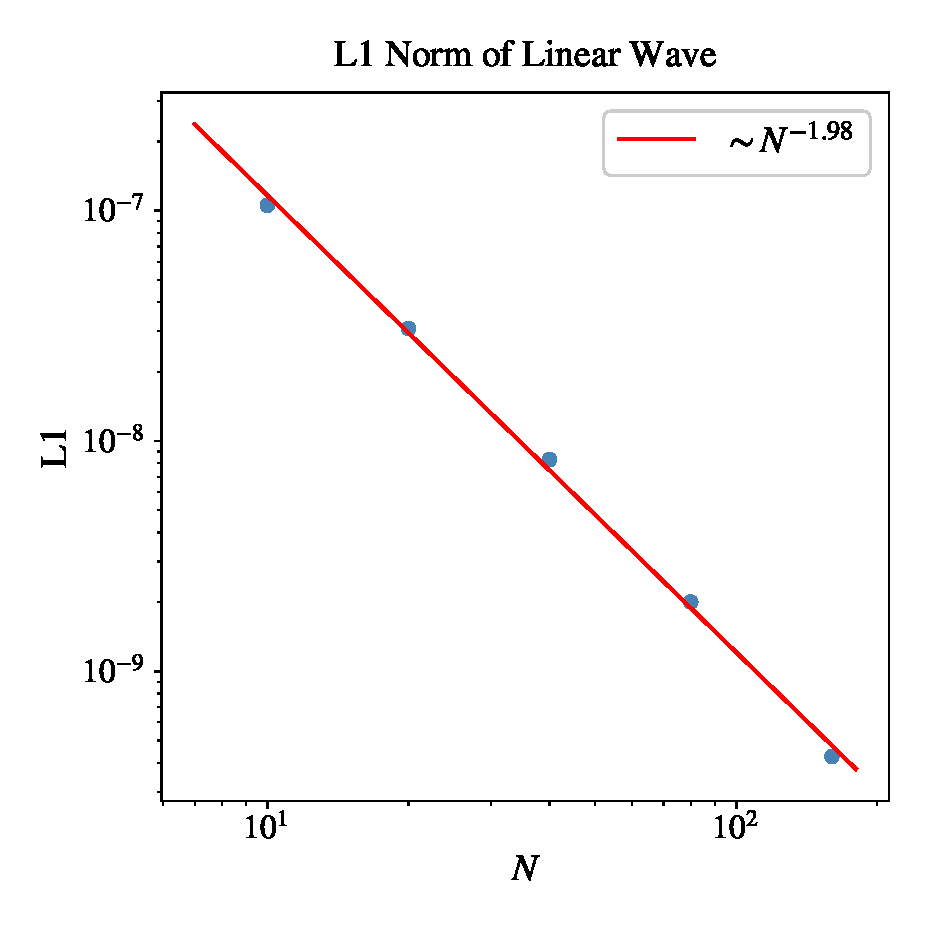
\includegraphics[width=0.4\textwidth]{figures/linear-wave-l1.eps}
        \caption{L1 norm of linear wave problem in 2d. Blue points are results
        of simulation from different resolutions overlaid by a linear fit showing
        the convergence is approximately second order.}
        \label{fig.linear-wave}
    \end{center}
\end{figure}
Figure \ref{fig.linear-wave} shows the $L1$ norm as a function of grid cells per dimension.
As expected, the convergence rate is approximately second order in time and space for
this smooth problem. In the presence of shocks or other discontinuities it is not expected
to have such convergence.

\subsubsection{Sod shock tube}
To examine the ability of the code to handle shock propagation we perform the Sod shock tube problem. The problem
consists of two different constant states at rest separated at the midpoint of the x axis. A discontinuity
exist in the density and pressure at the midpoint. At $t=0$ the high density region flows into the
lower density region. The flow produces a rarefaction, contact discontinuity, and a shock wave emanating
from the density discontinuity. Thus, this problem creates a great test for the codes ability to capture the
three wave types.

For our initial setup we use a unit box with reflective boundary conditions, linear
reconstruction and the HLLC solver. The discontinuity lies along the x axis at 0.5.
The density and pressure are defined as follows
\begin{equation}
	\rho = \left\{
      \begin{array}{@{}ll@{}}
        	1.0 & \text{for}\ x \leq 0.5 \\
            0.125 & \text{for}\ x > 0.5
    	\end{array}\right.
\end{equation}
and
\begin{equation}
	P = \left\{
      \begin{array}{@{}ll@{}}
        	1.0 & \text{for}\ x \leq 0.5 \\
            0.1 & \text{for}\ x > 0.5
    	\end{array}\right.
\end{equation}
with $\gamma = 1.4$. The particles are laid out in a Cartesian grid and the simulation is evolved
until $t=0.15$. The number of particles per dimension is chosen to be $N=100$ and $N=45$ for 2D
and 3D respectively. This allows a comparison of a high and low resolution run.
\begin{figure}
    \begin{center}
        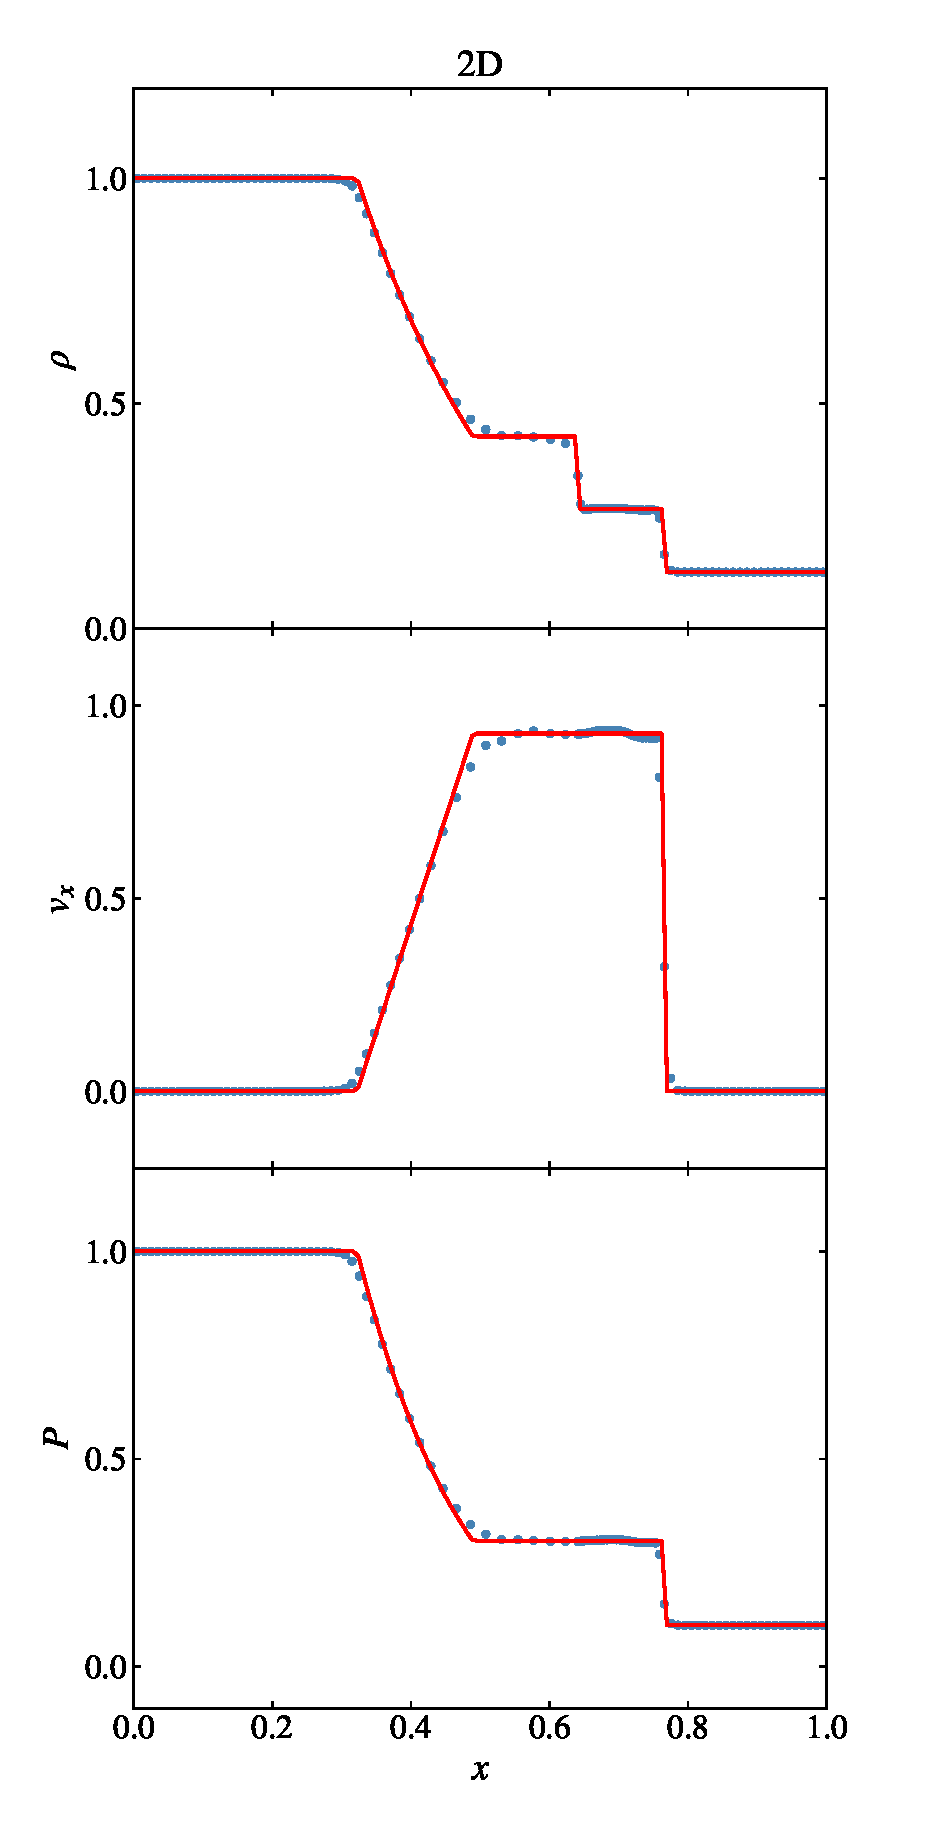
\includegraphics[width=0.4\textwidth]{figures/sod_2d.eps}
        \includegraphics[width=0.4\textwidth]{figures/sod_3d.eps}
        \caption{Profiles of density, x-component of the velocity and pressure of the Sod simulation. Left 2D run using 
        a total of $100\times100$ particles. Right 3D run using a total of $45\times45\times45$,
        we only plot a slice of particles defined by $z=0$.
        Light blue points are the simulation while the red line is the exact solution.}
        \label{fig.sod}
    \end{center}
\end{figure}
Figure \ref{fig.sod} plots the points of the simulation for density, x-component of
the velocity and pressure; only particles with $z=0$ are plotted for the 3D run. The red line is the analytical solution. For the 2D simulation we can see
the shock is well resolved as is the contact discontinuity. Further the Lagrangian nature of
the code can be seen as many particles have been squeezed between the contact discontinuity and the
shock front while particles in the rarefaction have been spread out. For the 3D, lower resolution
run, the code catches all three waves. Although, the contact discontinuity wave has been
smoothed.

\subsubsection{Explosion}
\begin{figure}
    \begin{center}
        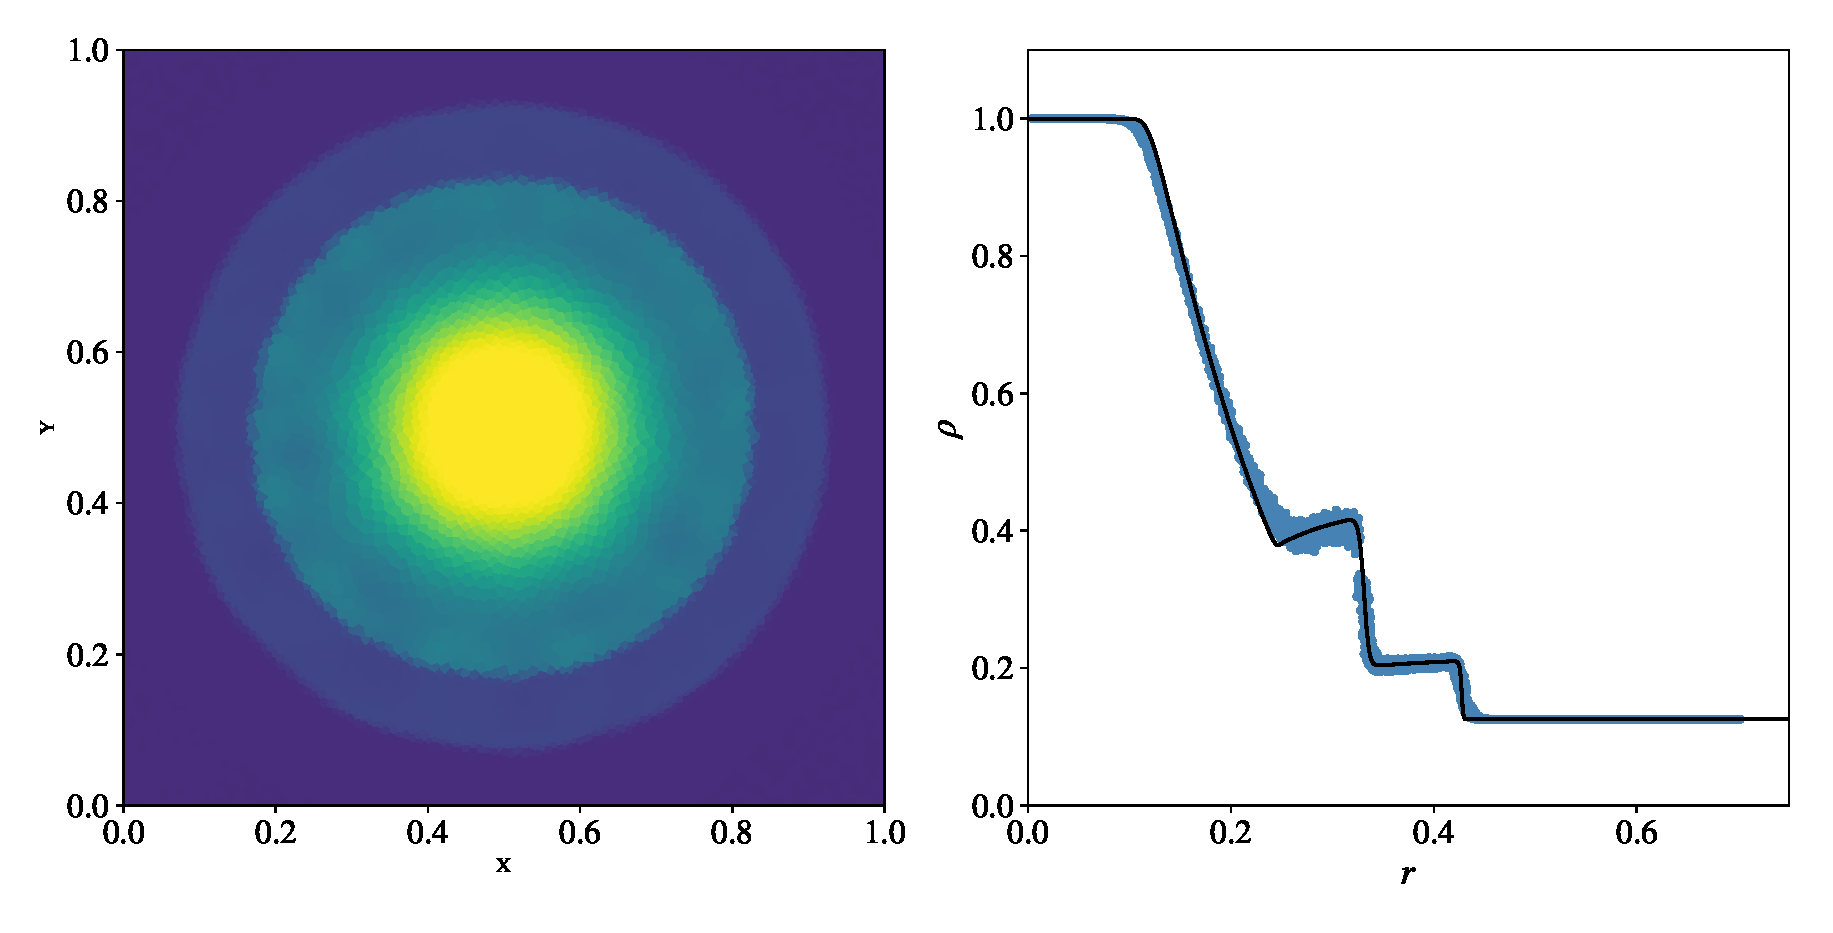
\includegraphics[width=0.9\textwidth]{figures/explosion_2d.eps}
        \caption{Density heatmap and radial profile of the Explosion problem. Left density
        heatmap, the irregular cells can been seen from the random initialization. Right
        radial density profile is an agreement with the exact solution in red.}
        \label{fig.explosion_2d}
    \end{center}
\end{figure}
An analog to the Sod problem is the 2D explosion problem. Like the Sod problem, the domain
is partition into two constant regions. However, the higher density region is now a circular
region of radius $r$ centered in a unit box. Similar to the Sod problem, the initial 
conditions generate a shock, contact discontinuity and rarefaction wave. However, in this case
the waves are now a circular shock wave traveling radially outward, a circular contact
discontinuity traveling in the same direction, and a rarefaction wave traveling towards the
center.

We use the same values as the Sod problem except we restrict the higher density values onto
the center of domain with radius $r=0.25$. Further, instead of using a Cartesian grid we sample
particles uniformly for a unit square and perform 10 iterations of Lloyds algorithm. 

Figure \ref{fig.explosion_2d} shows the density map and density profile. Clearly the cells
density matches the analytical solution in red. Further, the solution captures all three waves
even though the mesh was built in a random fashion. This an important difference over Eulerian
codes, since Lagrangian codes are not constrained to any initial particle placement. Therefore
one can reach better accuracy by placing the particles in way that exploits the problem. We will
see a later example of this in the Evrards problem.

\subsubsection{Gresho vortex}
Our next problem will test stability of the code. Gresho and Chan cite, introduced an interesting
problem to test for conservation of angular momentum. A vortex in a unit 2D box with constant 
density $\rho=1$ is setup with the following angular velocity
\begin{equation}
	v_\phi (r) = \left\{
      \begin{array}{@{}ll@{}}
        	5r & \text{for}\ 0 \leq r < 0.2 \\
            2-5r & \text{for}\ 0.2 \leq r < 0.4 \\
            0 &\text{for}\ \geq 0.4
    	\end{array}\right.
\end{equation}
The angular velocity of the vortex grows linearly as one moves radially outward from
the center until midway of the disk. Then the velocity decreases linearly until it
vanishes at the rim of the disk. This produces triangular shape velocity profile.
The corresponding pressure is
\begin{equation}
	P(r) = \left\{
      \begin{array}{@{}ll@{}}
        	5 + 25/2r^2 & \text{for}\ 0 \leq r < 0.2 \\
            9+25/2r^2 - 20r + 4\ln(r/0.2) & \text{for}\ 0.2 \leq r < 0.4 \\
            3 + 4\ln(2) &\text{for}\ \geq 0.4.
    	\end{array}\right.
\end{equation}
The pressure is chosen such that the pressure gradients balance the centrifugal forces
generated by the rotation. Thus producing a solution that is independent of time.
\begin{figure}
    \begin{center}
        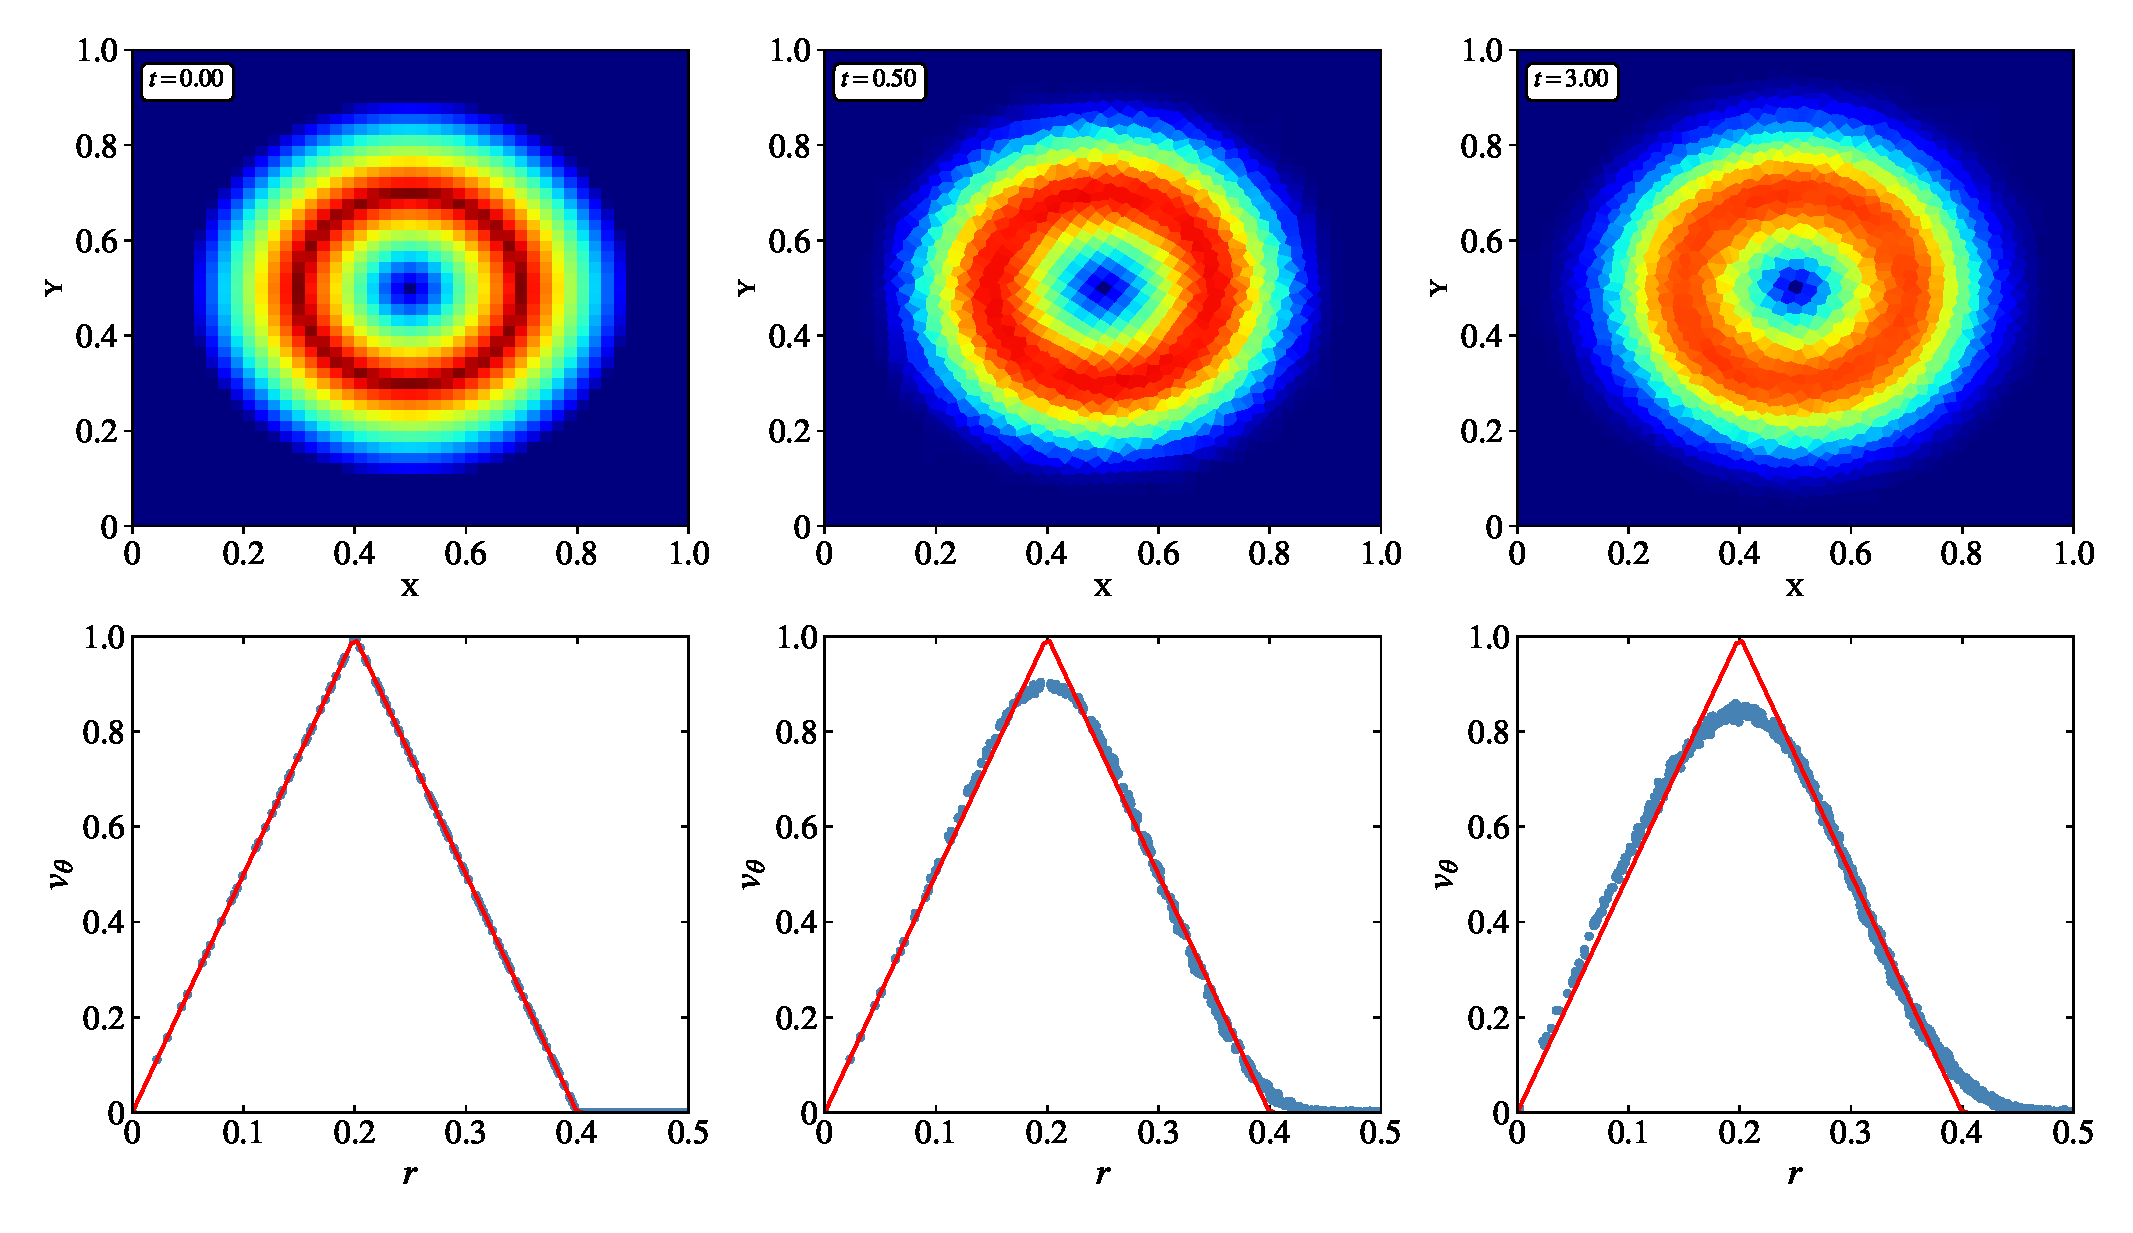
\includegraphics[width=0.9\textwidth]{figures/gresho_vortex.eps}
        \caption{Heatmap and radial profile of azimuthal velocity. Top row: time evolution
        of the cells at times $t=0.0, 0.5, 3.0$. Bottom row: radial profile of azimuthal
        velocity. As the simulation evolves the systems remains in equilibrium.}
        \label{fig.gresho_vortex}
    \end{center}
\end{figure}
Figure \ref{fig.gresho_vortex} shows three snapshots at $t=0.0, 0.5, 3.0$ of the azimuthal
velocity. The top row is a 2d heat map while the bottom row is a radial profile. At time $t=0$
all the cells are rectangular. As the system evolves the cells that are rotating become irregular 
polygons. There is a small amount of velocity smoothing at the initial largest velocities and at
the rim of the vortex. However it is evident that the system stays in equilibrium.

\subsubsection{Sedov-Taylor}
Another test generates a shock is the Sedov-Taylor blast wave problem. In this problem a homogeneous
gas is injected with a large amount of energy in a point-like region at the center of the domain.
A spherical shock is created emanating from the center. The shock propagates radially outward
sweeping mass into a thin shell and creating a cavity behind the shock. The problem has a well known
analytical self-similar solution cite. Applying the Rankine–Hugoniot at the shock front the density
jumps to a maximum compression of
\begin{equation}
	\rho_{\mathrm{max}}/\rho = (\gamma + 1)/(\gamma - 1),
\end{equation}
for $\gamma = 5/3$ this amounts to a max value of 4.

We consider the 2D and 3D case. A unit box is setup with particles in a Cartesian grid of size
$45\times 45$ and $45 \times 45 \times 45$ for 2D and 3D respectively. The stationary gas has
a constant density of $\rho = 1.0$ and pressure $P = 10^{-6}$ with $\gamma=5/3$. The simulation is
allowed to run to time $t=0.06$ using linear reconstruction and the HLLC solver.
\begin{figure}
    \begin{center}
        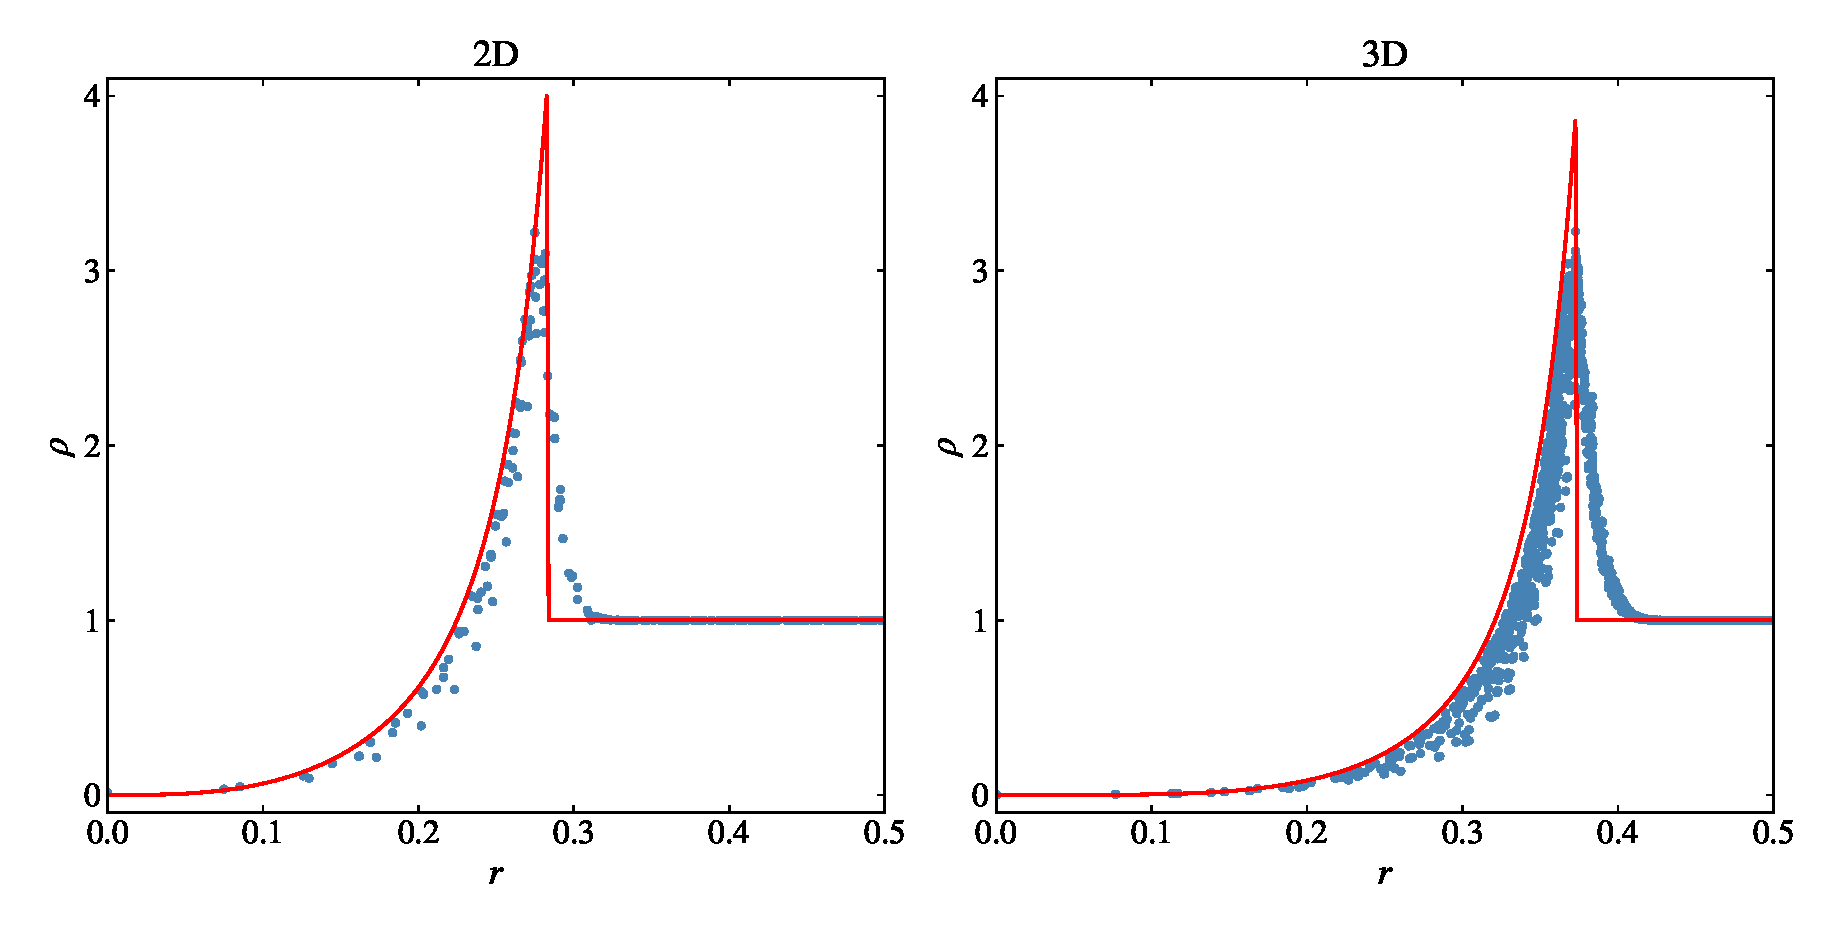
\includegraphics[width=0.9\textwidth]{figures/sedov_compare.eps}
        \caption{Density profile of Sedov-Taylor blast wave problem. Left is the 2D version with an initially
        Cartesian mesh of $45 \times 45$. Right is the 3D version with an initially Cartesian mesh of 
        $45 \times 45 \times 45$. Light blue points are the density a radius $r$ from the center of the explosion
        while the red line is the exact solution.}
        \label{fig.sedov}
    \end{center}
\end{figure}
Figure \ref{fig.sedov} shows the cell density as a function of radial distance from the center of the
explosion. It is noted that shock is well resolved by the cells as the mesh has deformed in such a way
that the shock front contains a large amount of cells which is evident in
Figure \ref{fig.sedov_panel}.
\begin{figure}
    \begin{center}
        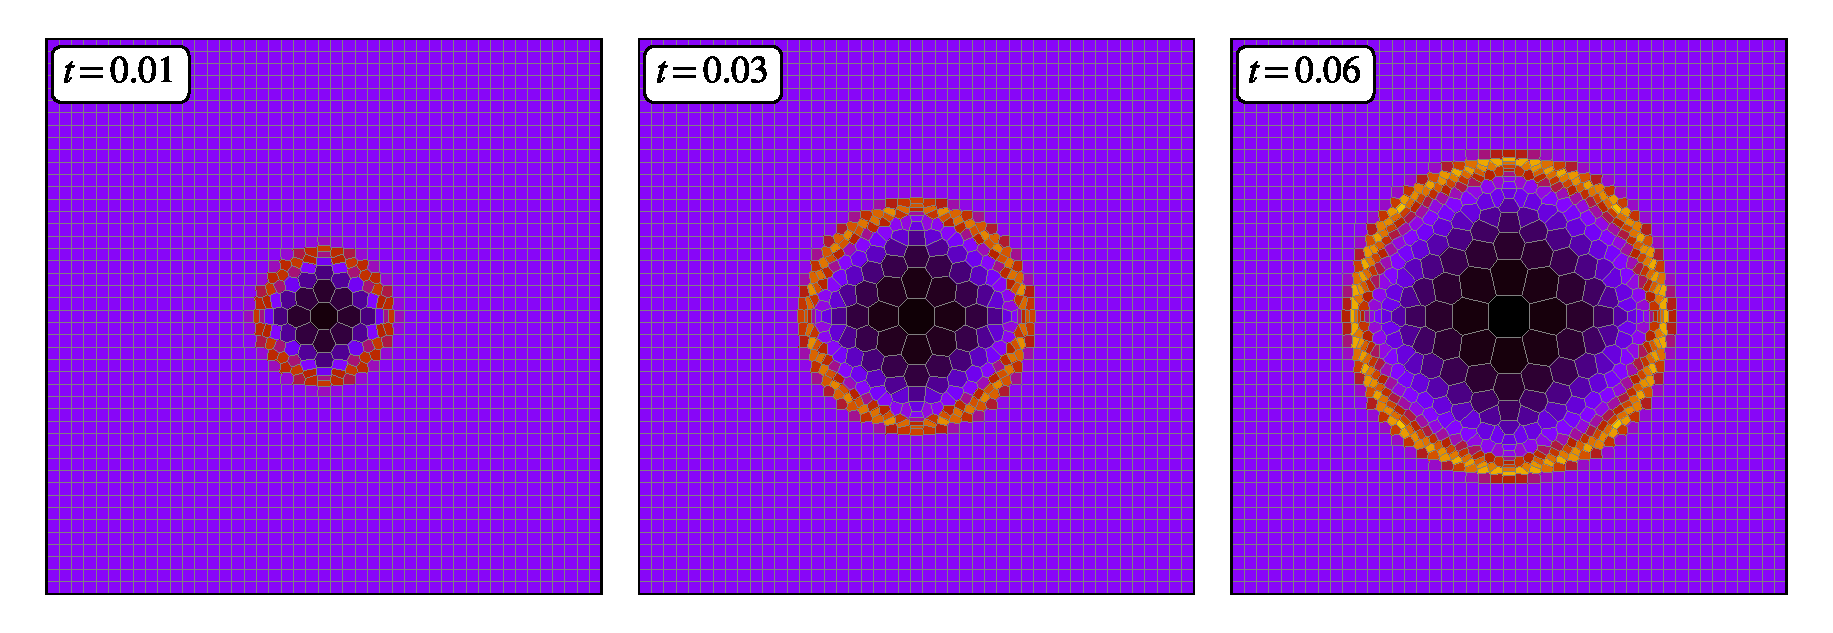
\includegraphics[width=0.9\textwidth]{figures/sedov_panel.eps}
        \caption{Evolution of the density at several times. The initial cell with the energy
        imparted remains stationary as the cells around it move radially outward. The cells at
        the shock are compressed allowing for better resolution.}
        \label{fig.sedov_panel}
    \end{center}
\end{figure}
The center cell, where the energy is deposited, remains stationary while the
cells around it move radially outward. The cells exterior to the shock remain
stationary until they are swept and compressed by the shock.

\subsubsection{Kelvin-Helmholtz}

\subsection{Gravity Tests}
\subsubsection{Two body}
Our first problem, in testing our gravity solver, is a simple two body problem where two particles
interact with each other through their gravitational force. Although, this problem does not really test the 
implementation of the gravity tree, since only two leaves will be constructed
in the tree and it is most likely that the leaves will interact with each other bypassing the node 
moments, it does test the gravity kernel and stability of the leap frog integrator.

For this problem an exact solution exists by reducing it to a single body. Given
two particles with masses $m_1$ and $m_2$ with positions $\vec{r}_1$ and $\vec{r}_2$ the equation of motion for
the reduced mass
\begin{equation}
	\frac{1}{\mu} = \frac{1}{m_1} + \frac{1}{m_2}
\end{equation}
is
\begin{equation}
	\mu\frac{d^2 \vec{r}}{dt^2} = -\frac{G m_1 m_2}{r^2}\hat{r},
    \label{eq.reduced-force}
\end{equation}
where $\vec{r}$ is the separation vector $\vec{r}_1 - \vec{r}_2$. Equation \ref{eq.reduced-force} can be
transformed to polar coordinates giving the solution
\begin{equation}
	r = \frac{a(1-\epsilon^2)}{1-\epsilon cos(\theta)}
\end{equation}
for initial conditions $a$ and $\epsilon$. The overall system evolves with a period of
\begin{equation}
    T = \sqrt{\frac{4\pi^2 a^3}{G m}},
\end{equation}
where $m=m_1 + m_2$. To recover the particles positions, a final transformation
of the form
\begin{equation}
	\begin{array}{rcl}
		\vec{r}_1 & = & \frac{m_1}{m}\vec{r}\\
    	\vec{r}_2 & = & -\frac{m_2}{m}\vec{r}
    \end{array}
\end{equation}
is used. The initial position and velocity of the particles can be parameterized by $a$,
$\epsilon$ and $q=m_1/m_2$
\begin{equation}
	\begin{array}{rcl}
    	\vec{r}_1 & = & a\frac{1-\epsilon}{1+q} \hat{x}\\
        \vec{v}_1 & = & \frac{1}{1+q}\sqrt{\frac{1+\epsilon}{1-\epsilon}}\sqrt{\frac{Gm}{a}} \hat{y}\\
        \vec{r}_2 & = & -q \vec{r}_1\\
        \vec{v}_2 & = & -q \vec{v}_1.
    \end{array}
\end{equation}

We setup the particles with parameter values $a=0.5$ and $\epsilon=0.25/0.75$ with $G=1$ and allow
the simulation to evolve for 10 periods. The time step is held fixed with a value of $dt=T/1000$.
In Figure \ref{fig.two_body} we show the trajectory for both particles as well as the evolution of
the relative total energy error. We clearly see that both trajectories remain along the exact solution
signifying the stability of the leap frog integrator. Further we see that the relative total energy
error remains bounded by zero and $-1.1\times10^{-4}$ indicating that the total energy remains
accurately conserved.
\begin{figure}
    \begin{center}
        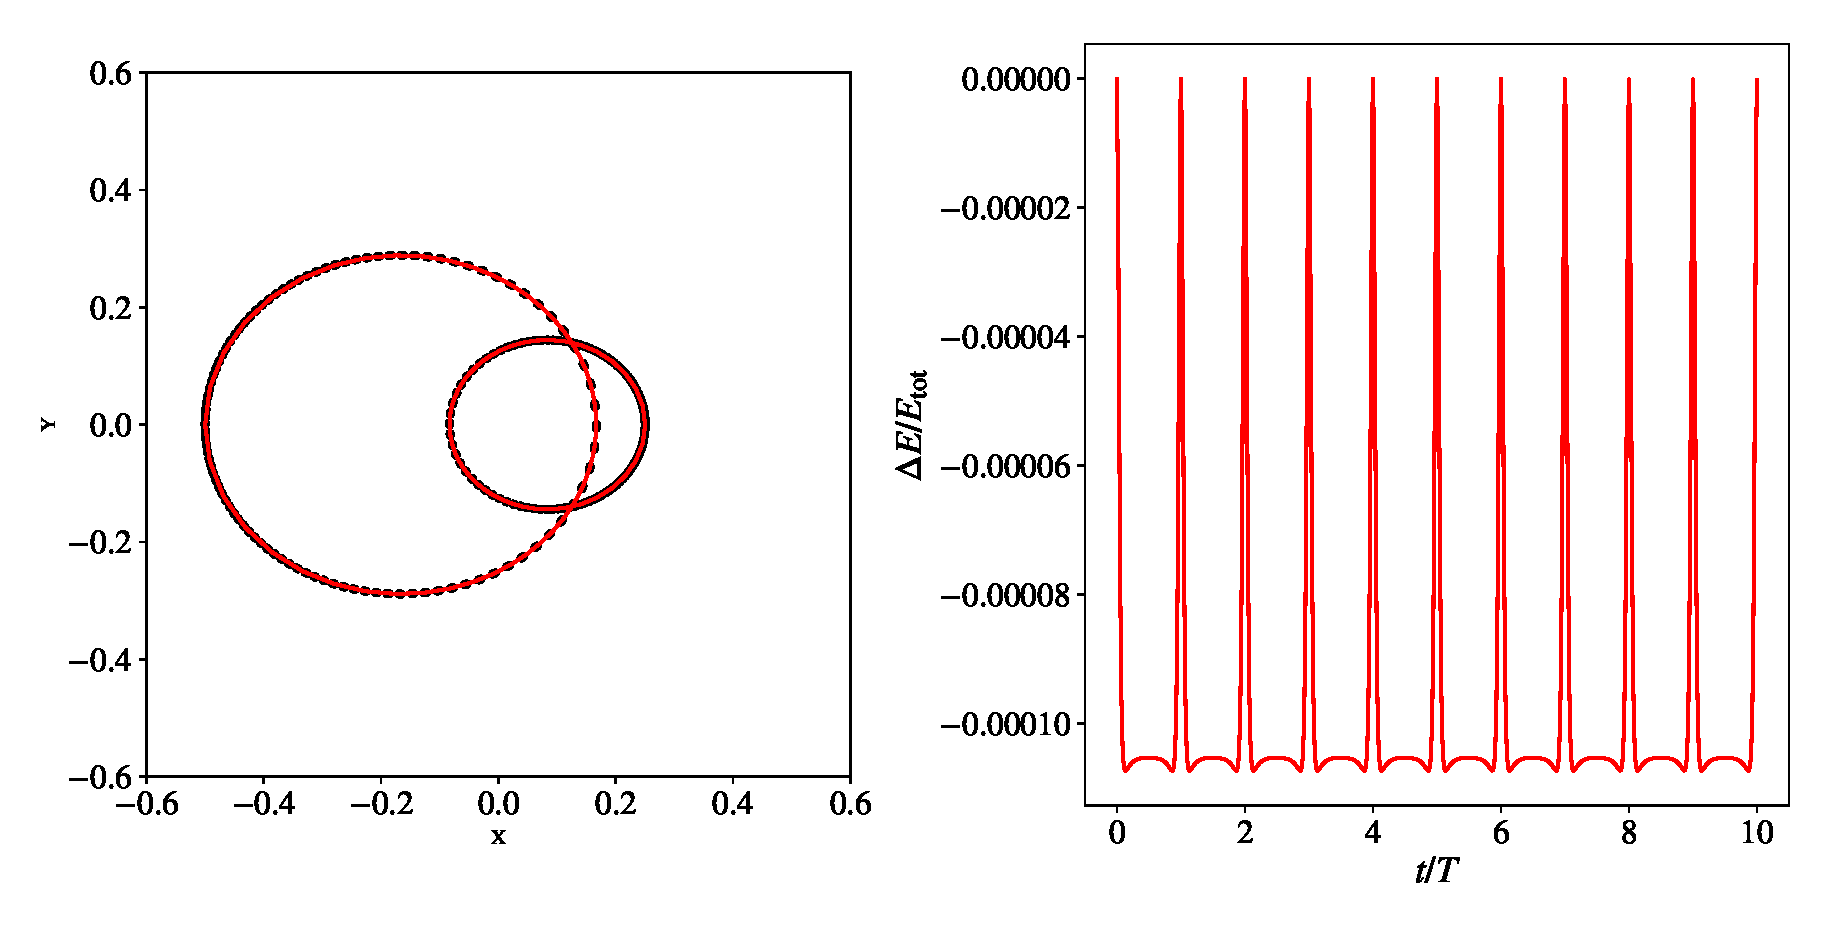
\includegraphics[width=0.9\textwidth]{figures/two_body.eps}
        \caption{Left: Trajectories of the two body problem for ten periods. Clearly
        both particles remain in their orbital path shown in red signifying the stability
        of the leap frog integrator. Right: Corresponding relative total energy error.
        The total energy remains accurately conserved as the worst relative error is
        $-1.1\times10^{4}$.}
        \label{fig.two_body}
    \end{center}
\end{figure}

\subsubsection{Plummer sphere}
The Plummer sphere cite is a model that can be used to describe the distribution of stars and in a cluster
and is commonly used to test gravity solvers. The Plummer sphere, i.e. a polytrope of index 5,
has a density profile of the from
\begin{equation}
	\rho (r) = \frac{3 M}{4\pi R^3} \left(1 + (r/R)^2\right)^{-5/2},
    \label{eq.plummer}
\end{equation}
where $M$ is the total mass of the cluster and $R$ is a scale parameter which sets the
size of the cluster. The system is in steady state with an isotropic velocity distribution.
To test our gravity solver, we initialize our particles with the given distributions and
advance the system in time. We expect the system to stay in steady state therefore we compare
the initial density distribution with the final state of the system.

For our test we chose the parameters of the Plummer sphere to be $M=1,000$ and $R=1$ with
$G=1$. We then sampled 10,000 particles using the the rejection technique outlined in
cite to set the position and velocities. The system is allowed to evolve to time $t=1$
which is roughly ten dynamical times. The gravitational tree used an opening angle 0.4
and smoothing parameter of 0.03.
\begin{figure}
    \begin{center}
        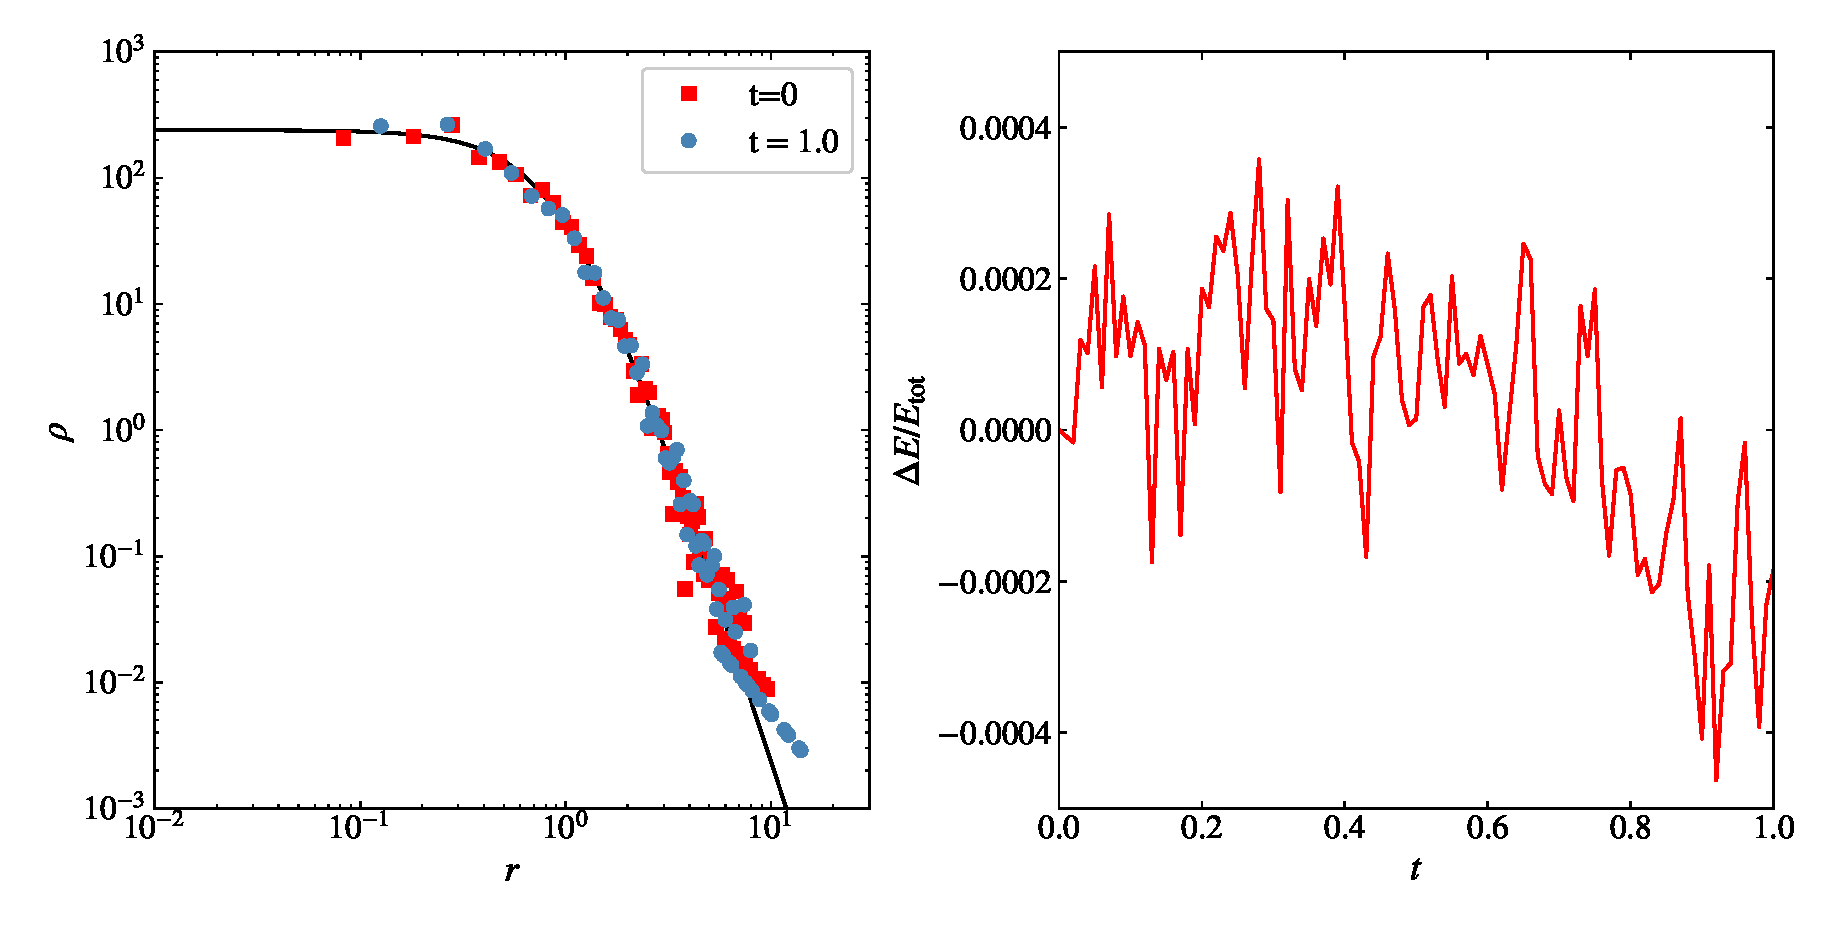
\includegraphics[width=0.9\textwidth]{figures/plummer.eps}
        \caption{Density profile of Sedov-Taylor blast wave problem. Left is the 2D version with an initially
        Cartesian mesh of $45 \times 45$. Right is the 3D version with an initially Cartesian mesh of 
        $45 \times 45 \times 45$. Light blue points are the density a radius $r$ from the center of the explosion
        while the red line is the exact solution.}
        \label{fig.plummer}
    \end{center}
\end{figure}
The left panel of Figure \ref{fig.plummer} shows the density profile at the initial and final 
time of the simulation with equation \ref{eq.plummer} overlaid as a reference. The density is calculated
by dividing the space by spherical shells, binning and dividing by the volume. It is clearly shown that
at the final time the particles remain in steady state with their positions matching the initial
distribution. The right panel of \ref{fig.plummer} shows the evolution of the relative error of the
total energy of the system. The error stays well below $5\times 10^{-4}$ with a final error of
$2\times 10^{-4}$, entailing the solver has accurately maintained the total energy.

\subsubsection{Rayleigh Taylor}
Our first hydrodynamic problem to include gravity is the Rayleigh Taylor instability problem.
The problem consists of dense fluid over a lighter fluid in the presence of a uniform 
vertical gravitational field. A perturbation is placed in the vertical direction causing the
dense field to sink while the lighter rises through buoyancy.

A rectangular domain of the size $[1\times3]$ is chosen with the gravitational force in the
$y$-direction with strength of $g=1$. The initial setup of the density
is
\begin{equation}
	\rho = \left\{
      \begin{array}{@{}ll@{}}
            1 & \text{for}\ y \leq 1.5 \\
            2 & \text{for}\ 5 > 1.5,
    	\end{array}\right.
\end{equation}
while the pressure is
\begin{equation}
	P = \left\{
      \begin{array}{@{}ll@{}}
            10 - y & \text{for}\ y \leq 1.5 \\
            11.5 + 2(y-1.5) & \text{for}\ 5 > 1.5,
    	\end{array}\right.
\end{equation}
such that the system is initially in hydrostatic equilibrium. A perturbation is applied
to the $y$-velocity
\begin{equation}
	v_y = \mathrm{cos}\left(2\pi x\right)\exp{-(y-1.5)^2/0.1}
\end{equation}
We set $\gamma=1$ and let the system evolve to $t=3.0$. Although without an implementation
of viscosity there is no one correct solution that all codes converge to. However, we can
visually inspect if our simulation share the same characteristics of another established
code. In Figure we that the single mode is very similar to the results from cite
\begin{figure}
    \begin{center}
        \includegraphics[width=0.6\textwidth]{figures/rayleigh_compare.eps}
        \caption{Density profile of Sedov-Taylor blast wave problem. Left is the 2D version with an initially
        Cartesian mesh of $45 \times 45$. Right is the 3D version with an initially Cartesian mesh of 
        $45 \times 45 \times 45$. Light blue points are the density a radius $r$ from the center of the explosion
        while the red line is the exact solution.}
        \label{fig.rayleigh}
    \end{center}
\end{figure}

We see the mode has the characteristics of

\subsubsection{Evrard Collapse}
The final test is the Evrards collapse problem which tests the coupling of self-gravity and hydrodynamics.
The problem consists of an initially non-rotating isothermal gas sphere with mass $M=1$ and radius $R=1$
with a density 
\begin{equation}
	\rho(r) = \left\{
      \begin{array}{@{}ll@{}}
            1/\left(2\pi r\right) & \text{for}\ r \leq 1 \\
            0 & \text{for}\ r > 1
    	\end{array}\right.
\end{equation}
and pressure
\begin{equation}
	P(r) = \left\{
      \begin{array}{@{}ll@{}}
            0.05 /\left(3\pi r\right) & \text{for}\ r \leq 1 \\
            0 & \text{for}\ r > 1.
    	\end{array}\right.
\end{equation}
The gravitational constant is set to $G=1$ and $\gamma=5/3$. The evolution of the sphere begins
with mass falling towards the center due to self-gravity. The pressure at the center rises and
produces a shock traveling outward through the in-falling gas. The final state of the gas is a
spherical distribution in hydrostatic virial equilibrium.

We setup an initial Cartesian grid of size $33\times 33\times 33$ particles. Due to the nature
of the $1/r$ density profile, a Cartesian mesh will not resolve the high density values unless
the resolution is sufficiently increased. However we have complete freedom on how to the particles
are initially setup. Therefore, we transform particles radially inside the sphere by the following
\begin{equation}
    r_{\mathrm{new}} = r_{\mathrm{old}}^{3/2}.
\end{equation}
Such a transformation maps a grid of equally spaced particles with uniform density to
a set of particles spaced in such a way that the uniform density follows a $1/r$ profile. 
\begin{figure}
    \begin{center}
        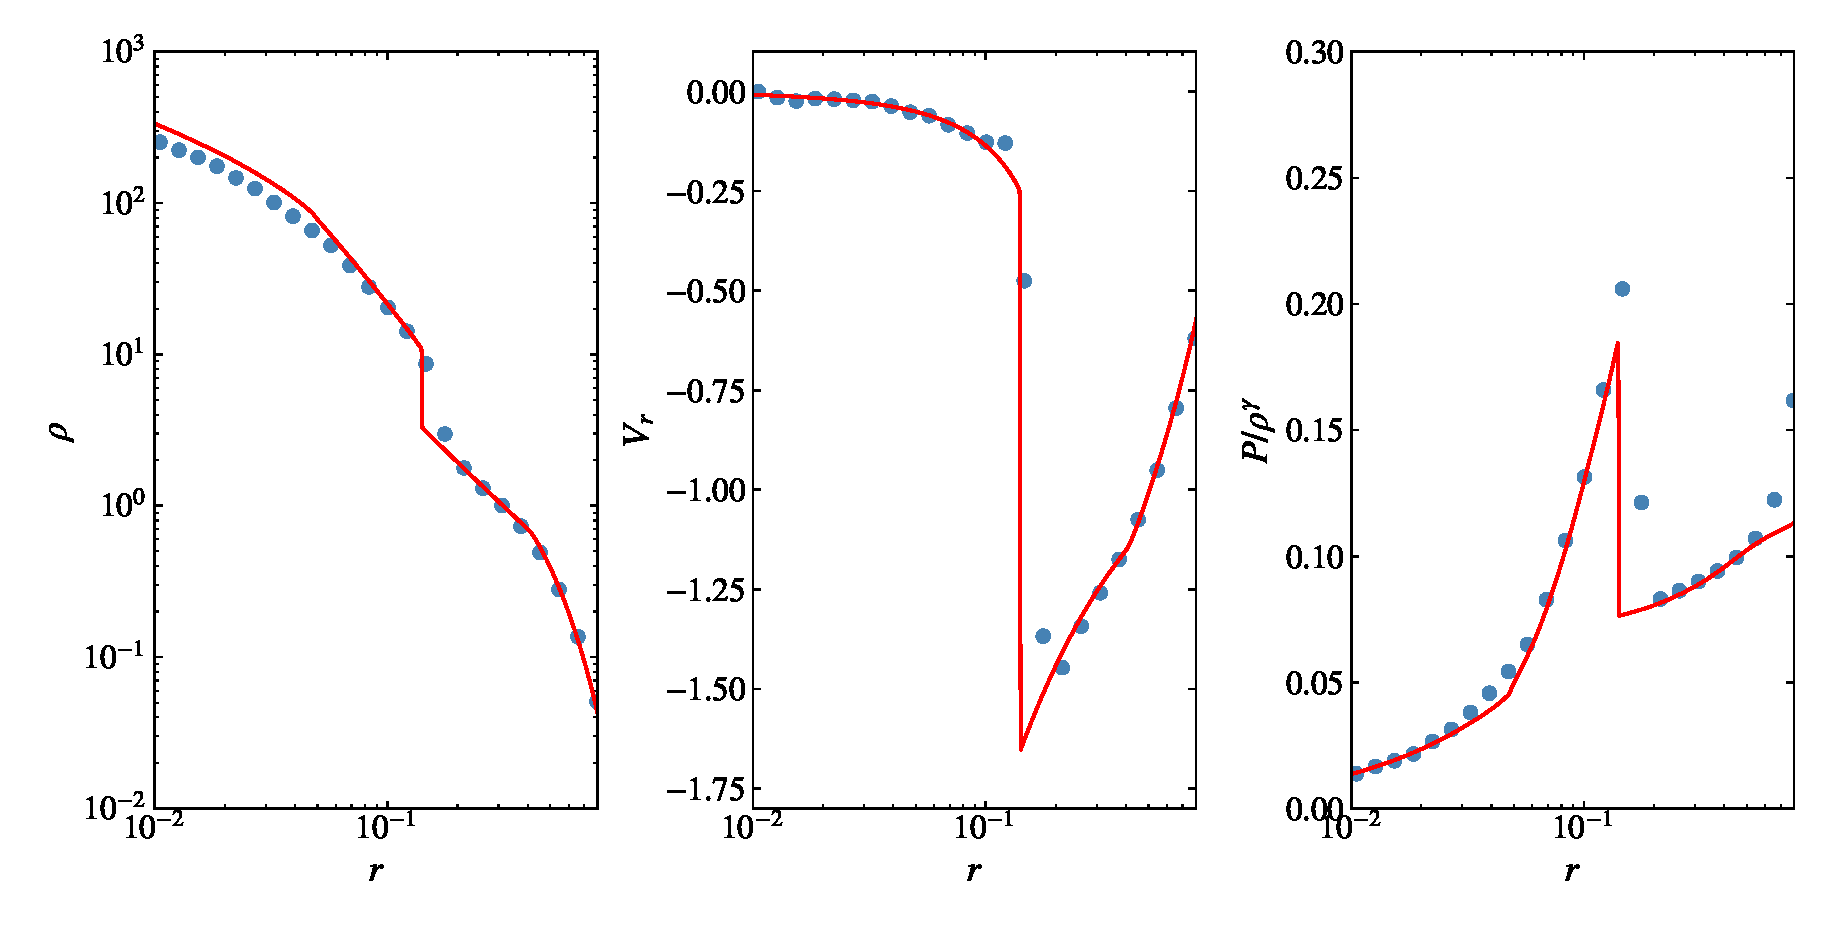
\includegraphics[width=0.9\textwidth]{figures/evrard.eps}
        \caption{Density profile of Sedov-Taylor blast wave problem. Left is the 2D version with an initially
        Cartesian mesh of $45 \times 45$. Right is the 3D version with an initially Cartesian mesh of 
        $45 \times 45 \times 45$. Light blue points are the density a radius $r$ from the center of the explosion
        while the red line is the exact solution.}
        \label{fig.evrard}
    \end{center}
\end{figure}

The radial averaged density, radial velocity and entropy are shown in Figure at time $t=0.81$
when the shock has formed and is traveling outward. We see all profiles adequately follow the
exact solution in red for this low resolution run. Further we see that there is significant
error in the conservation of energy Figure. This is expected as noted by Springel. The 
discrepancy arises from the gravitational work term which ignores the motion of mass
exchanged by adjacent cells. Springel proposed a new formulation for then energy equation
that results in better energy conservation. This updated method will be added in the next
revision of the code.
\begin{figure}
    \begin{center}
        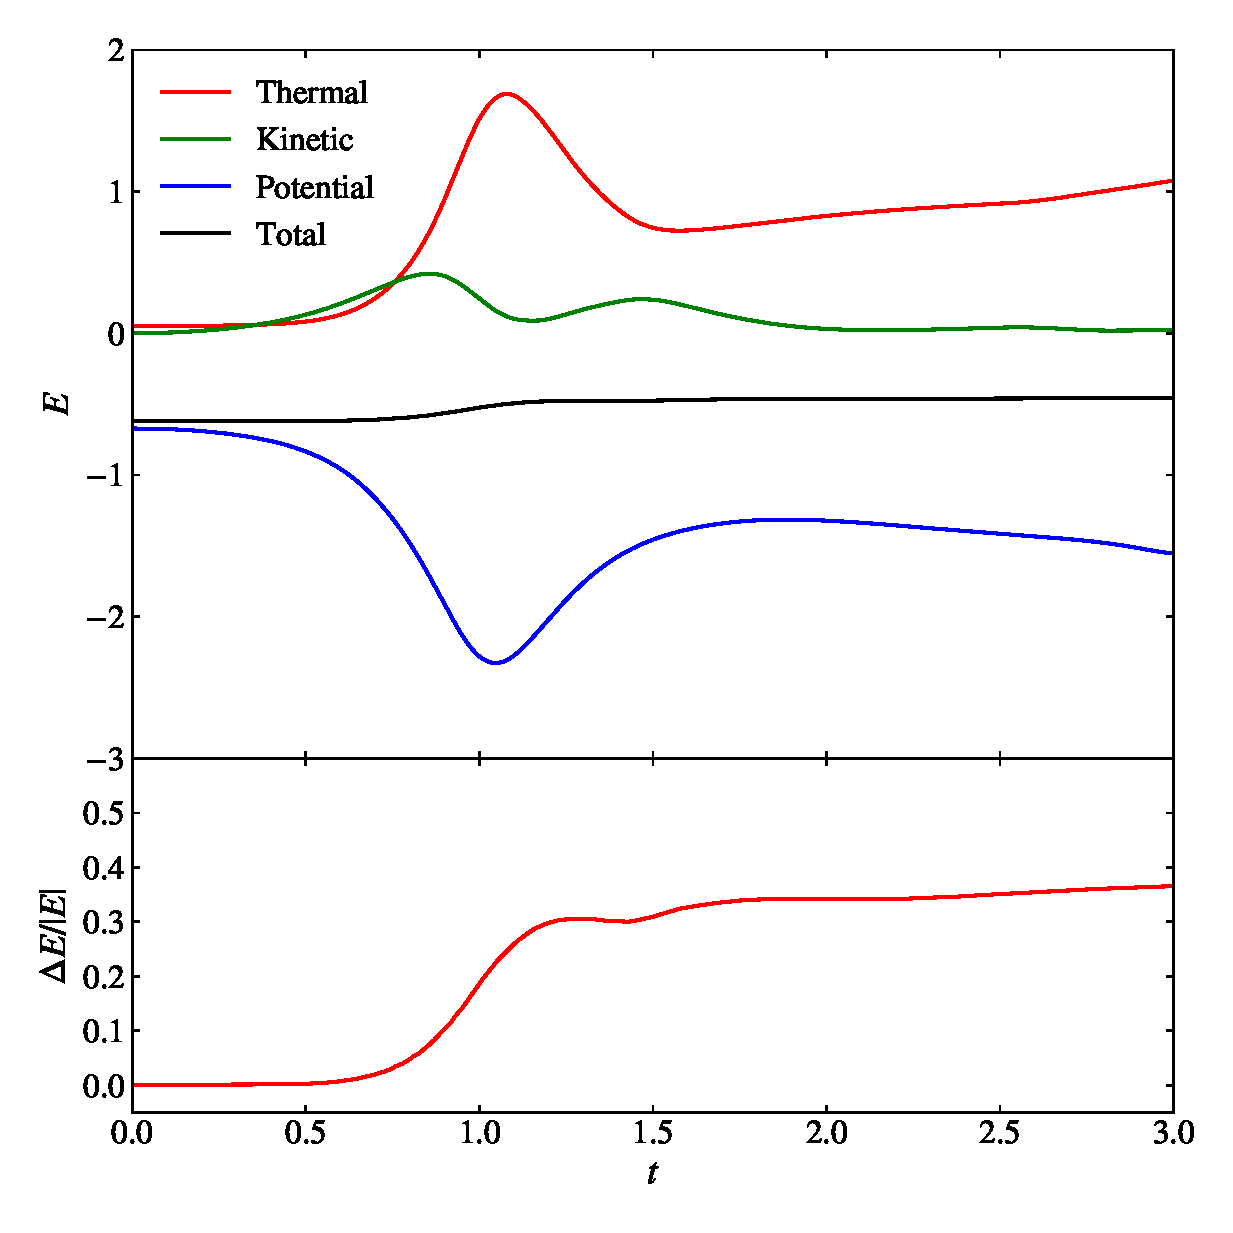
\includegraphics[width=0.6\textwidth]{figures/evrard_energy.eps}
        \caption{Density profile of Sedov-Taylor blast wave problem. Left is the 2D version with an initially
        Cartesian mesh of $45 \times 45$. Right is the 3D version with an initially Cartesian mesh of 
        $45 \times 45 \times 45$. Light blue points are the density a radius $r$ from the center of the explosion
        while the red line is the exact solution.}
        \label{fig.evrard_energy}
    \end{center}
\end{figure}
